\chapter{Introduzione}
La \textit{cefalometria} è uno strumento incomparabile di studio, di diagnosi, di pianificazione di trattamento e di valutazione della crescita, con o senza trattamento. Essa è principalmente usata in Ortodonzia, ma anche in Chirurgia Maxillo-Facciale, in Pedodonzia, in Protesi o in Chirurgia Plastica. Si tratta di un metodo con il quale si risale dall'effetto alla causa, dalla conseguenza al principio, dal particolare al generale o dal complicato al semplice per studiare i fattori di situazione in dettaglio. È per questa logica del ragionamento che noi possiamo tentare di scoprire la vera eziologia di alcune patologie, non rilevabile superficialmente.

Il concetto di normalità in biometria è una nozione difficile da definire, ma che potrebbe definirsi come appartenente alla norma statistica. La norma ideale corrisponde ai valori medi della media aritmetica. L'intervallo di dispersione della normalità è abbastanza vasto e raggruppa quasi il 70\% della popolazione di cui una delle estremità possiede delle tendenze Brachifacciali e l'altra delle tendenze Dolicofacciali.

È per questo motivo che, nel corso degli anni, alcuni Autori hanno ideato tecniche cefalometriche atte ad \textit{individualizzare} il processo diagnostico, non affidandosi più a medie statistiche di popolazione, ma sfruttando le proporzioni esistenti tra le varie componenti dell'apparato stomatognatico.

\section{La ``norma individuale''}

Con un appropriato utilizzo, i tracciati cefalometrici possono notevolmente migliorare la diagnosi e la pianificazione del trattamento ortodontico. Vengono però principalmente utilizzate per scopi descrittivi. Dei tracciati individuali vengono paragonati con un \textit{pattern facciale medio}, e le differenze richiedono una considerevole interpretazione. Bisogna tuttavia notare come le variazioni individuali nella posizione dei \textit{punti di repere} facciali rendano il \textit{pattern facciale medio} forse irreperibile nella popolazione, ma tuttavia un utile mezzo di riferimento anche se a rischio di incorrere in eccessiva semplificazione.

\begin{wrapfigure}{L}{.5\textwidth}
\centering
\fbox{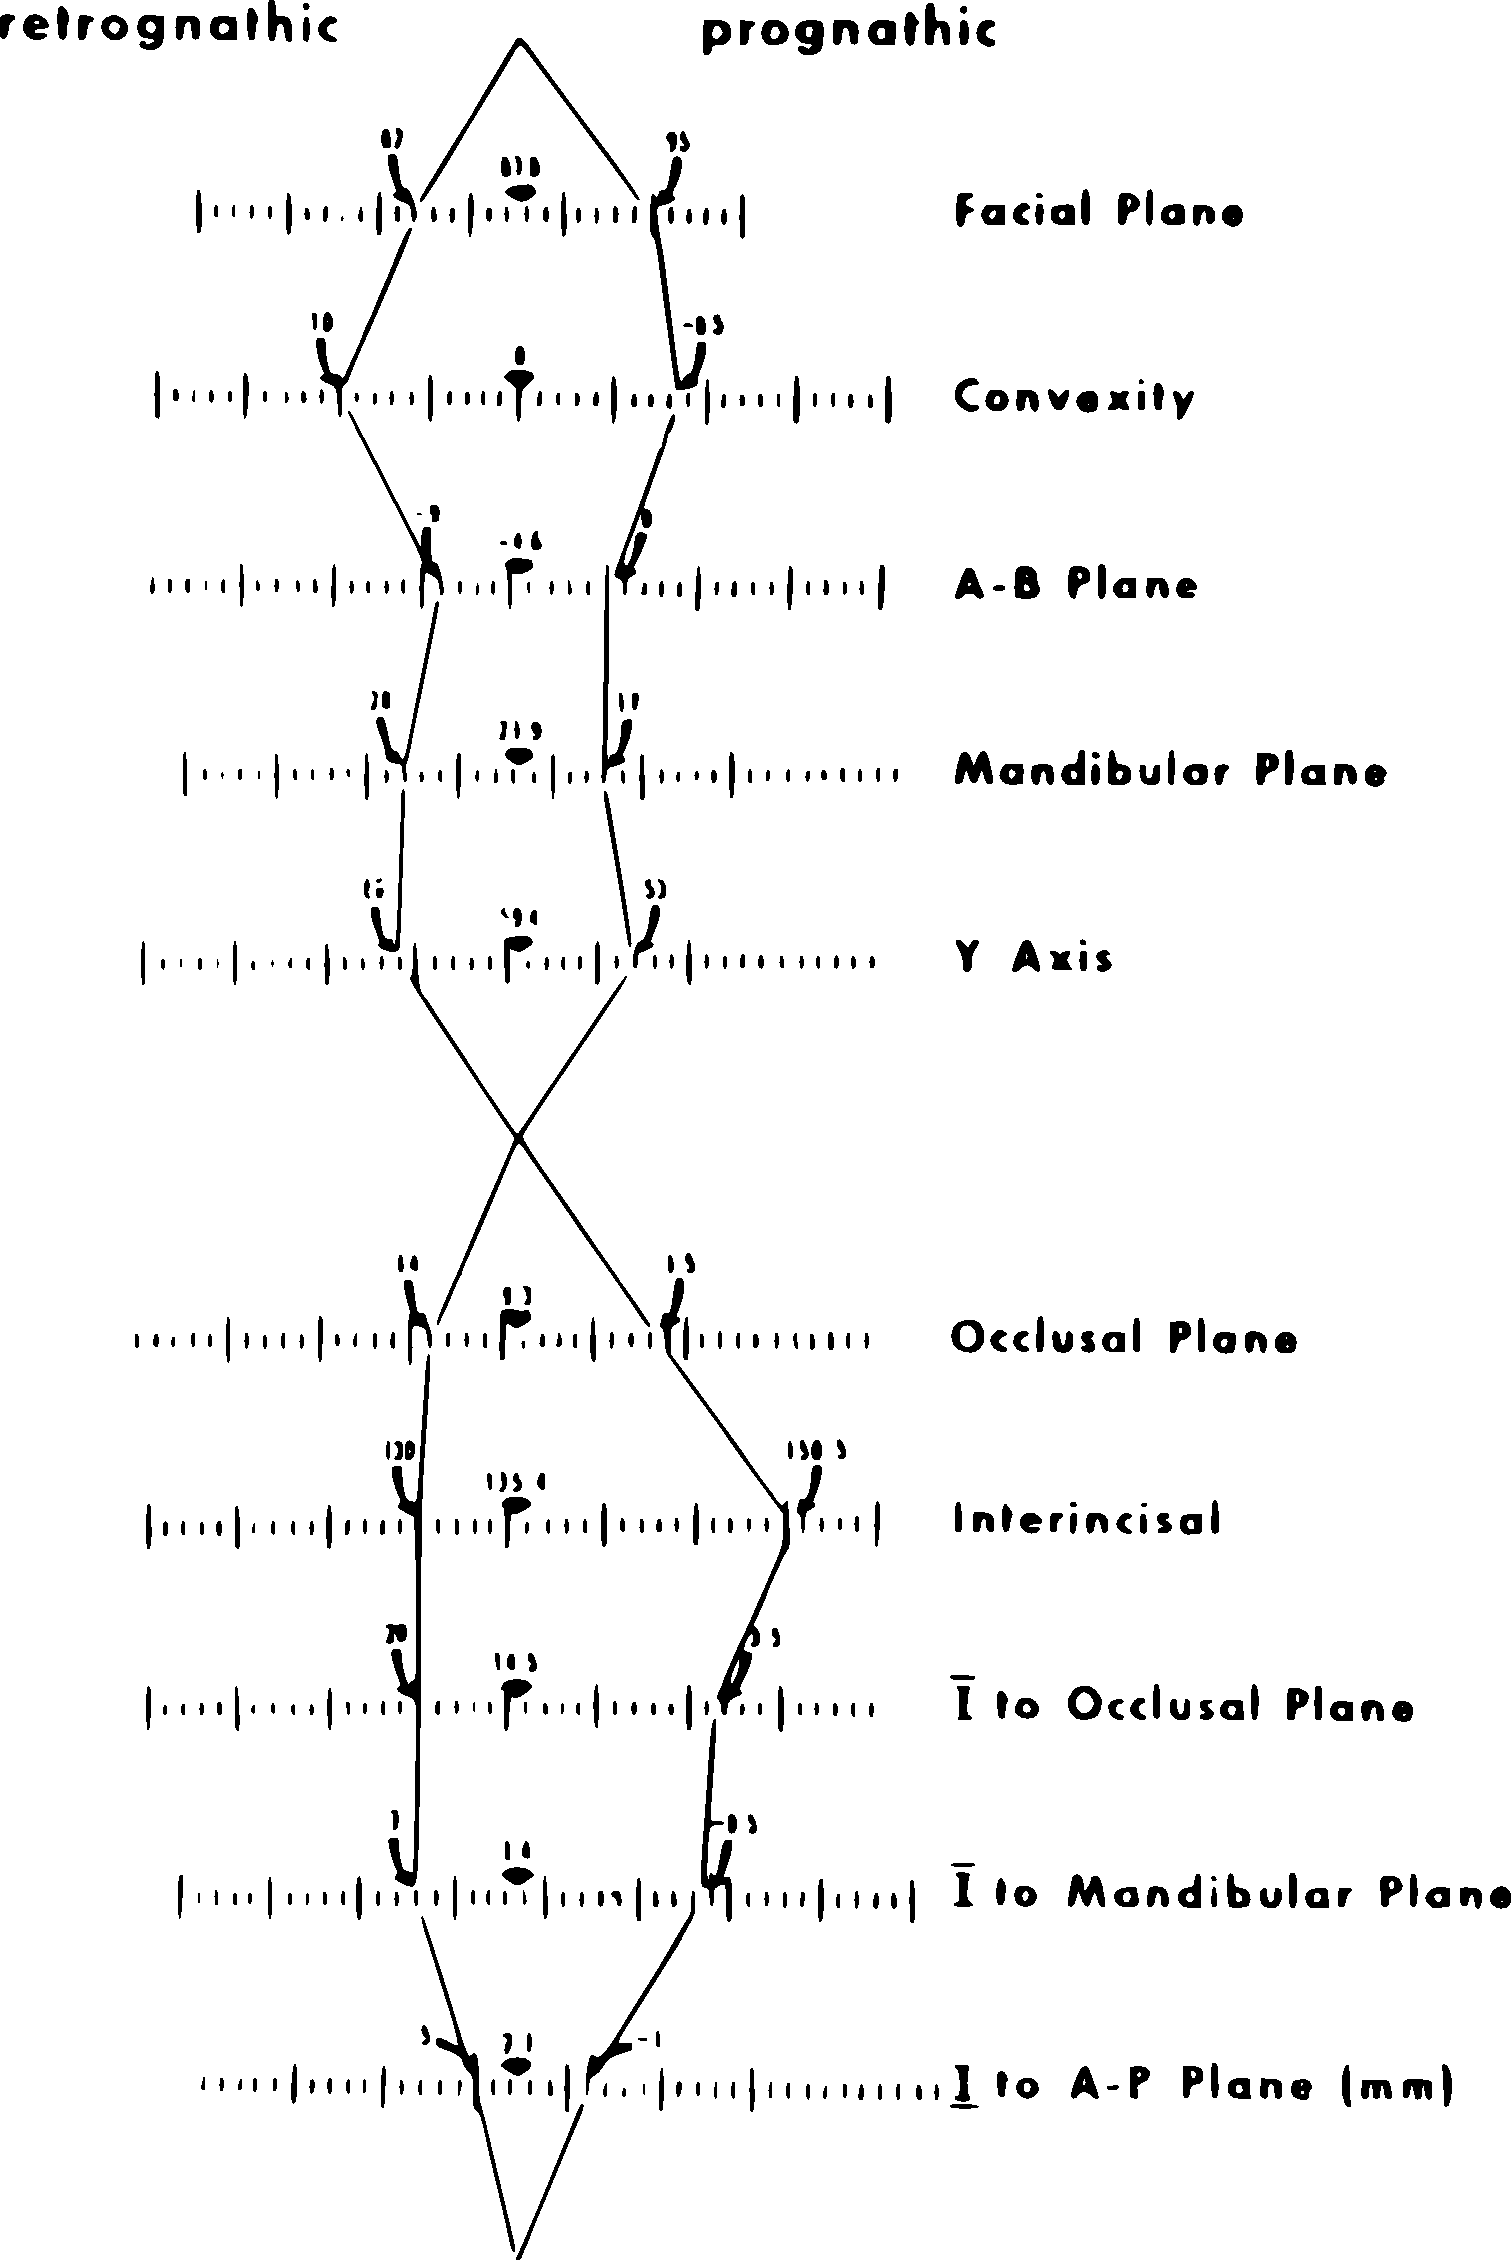
\includegraphics[width=.45\textwidth]{./images/downs.pdf}}
% downs.jpg: 1025x1440 pixel, 72dpi, 36.16x50.80 cm, bb=0 0 1025 1440
\caption{L'analisi di Downs enfatizza le variazione individuali dal pattern facciale medio. Può servire come una guida all'interpretazione di analisi cefalometriche per realizzare piani di trattamento più conformi alla realtà.}
\label{fig:downs}
\end{wrapfigure}

La prima analisi cefalometrica sviluppata negli Stati Uniti d'America fu quella di Downs\footnote{biblio 46}, che mirava ad illustrare la \textit{diffusione} di tutte le misure di un individuo, disegnando questi valori su un grafico a $\pm1$ e $\pm2$ deviazioni standard da una linea verticale che rappresentava il punto centrale della distribuzione di ogni variabile (fig. \ref{fig:downs}). Quest'analisi enfatizzò la consistenza delle differenze individuali attorno alla media statistica, e aiutò a sviluppare modelli di studio dello sviluppo individuale della faccia che erano spesso più realistici dei risultati cefalometrici.

Considerato che la correzione dei dismorfismi è basata sulla premessa che, con la normalizzazione della dentatura e della faccia, si migliori la funzionalità generale, la terapia è condizionata dalle caratteristiche individuali del pattern facciale del singolo paziente. In altre parole, è la \textbf{\textit{norma individuale}} a determinare il piano di trattamento, così come enfatizzato da Andresen nel 1931\footnote{biblio 47}.

Una volta riconosciuto il concetto di norma individuale, il processo diagnostico diventa un'equazione complessa. Diventa necessario identificare diverse incognite per determinare le indicazioni, e le controindicazioni, di un trattamento, e gli obiettivi dello stesso in termini di necessità e benefici. L'ortodonzista deve quindi valutare:

\begin{itemize}
\item l'impatto psicosociale dei cambiamenti dentofacciali;
\item l'impatto psicologico della malocclusione sulla funzionalità labiale, i movimenti mandibolari, la respirazione, la crescita e lo sviluppo, la masticazione e la salute orale;
\item gli aspetti anatomici del disallineamento dentale, dell'occlusione e delle relazioni dentali, della forma, disarmonia o dell'asimmetria facciale, e della configurazione dei tessuti molli.
\end{itemize}

In breve, la diagnosi deve basarsi sulla valutazione del paziente \textit{in toto}, non escludendo alcun ambito. La pianificazione del trattamento deve basarsi sul conseguimento di un \textit{optimum} estetico e funzionale per ogni singolo paziente, piuttosto che l'aderenza a norme codificate. L'occlusione ideale, e la divina proporzione, possono quindi essere, al più, degli indicatori della giusta direzione da intraprendere.

\section{Scopo della tesi, materiali e metodi}
Questo studio si propone quindi di presentare alcune tecniche di analisi cefalometrica, di seguito definite \textit{proporzionali}, e di valutarne il differente impatto in termini diagnostici, rispetto a quelle tecniche che si basano su \textit{valori ideali} comuni per tutti, statisticamente rilevati.

In particolare, verranno prese in esame le seguenti tecniche:
\begin{itemize}
\item analisi proporzionali
\begin{itemize}
\item analisi architetturale di Delaire
\item analisi delle controparti di Enlow
\item analisi proporzionale di Coben
\item la rosa dei venti di Sassouni
\end{itemize}
\item analisi statistiche
\begin{itemize}
\item Downs
\item Giannì
\item Ricketts
\item Steiner
\end{itemize}
\end{itemize}

Saranno prese in esame XXX teleradiografie in proiezione latero-laterale, e di ognuna verrà effettuato il tracciato cefalometrico, secondo le analisi di cui sopra. La comparazione tra le analisi si baserà sugli eventuali diversi risultati diagnostici (? XXX), che giustifichino la maggiore complessità delle analisi ``proporzionali''.
